\documentclass[tikz,border=0cm]{standalone}
\usepackage{type1cm}
\usepackage{fp}
\usetikzlibrary{calc}
\usetikzlibrary{shadows}

\usepackage{fetamont}
\usepackage{cmbright}

\usepackage{bm,amsmath,amssymb}
\usepackage{soul}
\usepackage{multirow}

\newcommand{\clm}{Cl\'{e}ment }
\newcommand{\norm}[1]{\lVert#1\rVert}

\definecolor{edblue}{RGB}{4, 80, 124}
\definecolor{eyellow}{RGB}{248, 176, 23}
\definecolor{elblue}{RGB}{55, 172, 195}

\usepackage[a4paper, margin=1in]{geometry}
\usepackage{url}
\usepackage{setspace}
\renewcommand{\baselinestretch}{1.0}
\let\OLDthebibliography\thebibliography
\renewcommand\thebibliography[1]{
  \OLDthebibliography{#1}
  \setlength{\parskip}{0pt}
  \setlength{\itemsep}{0pt plus 0.3ex}
}

\begin{document}

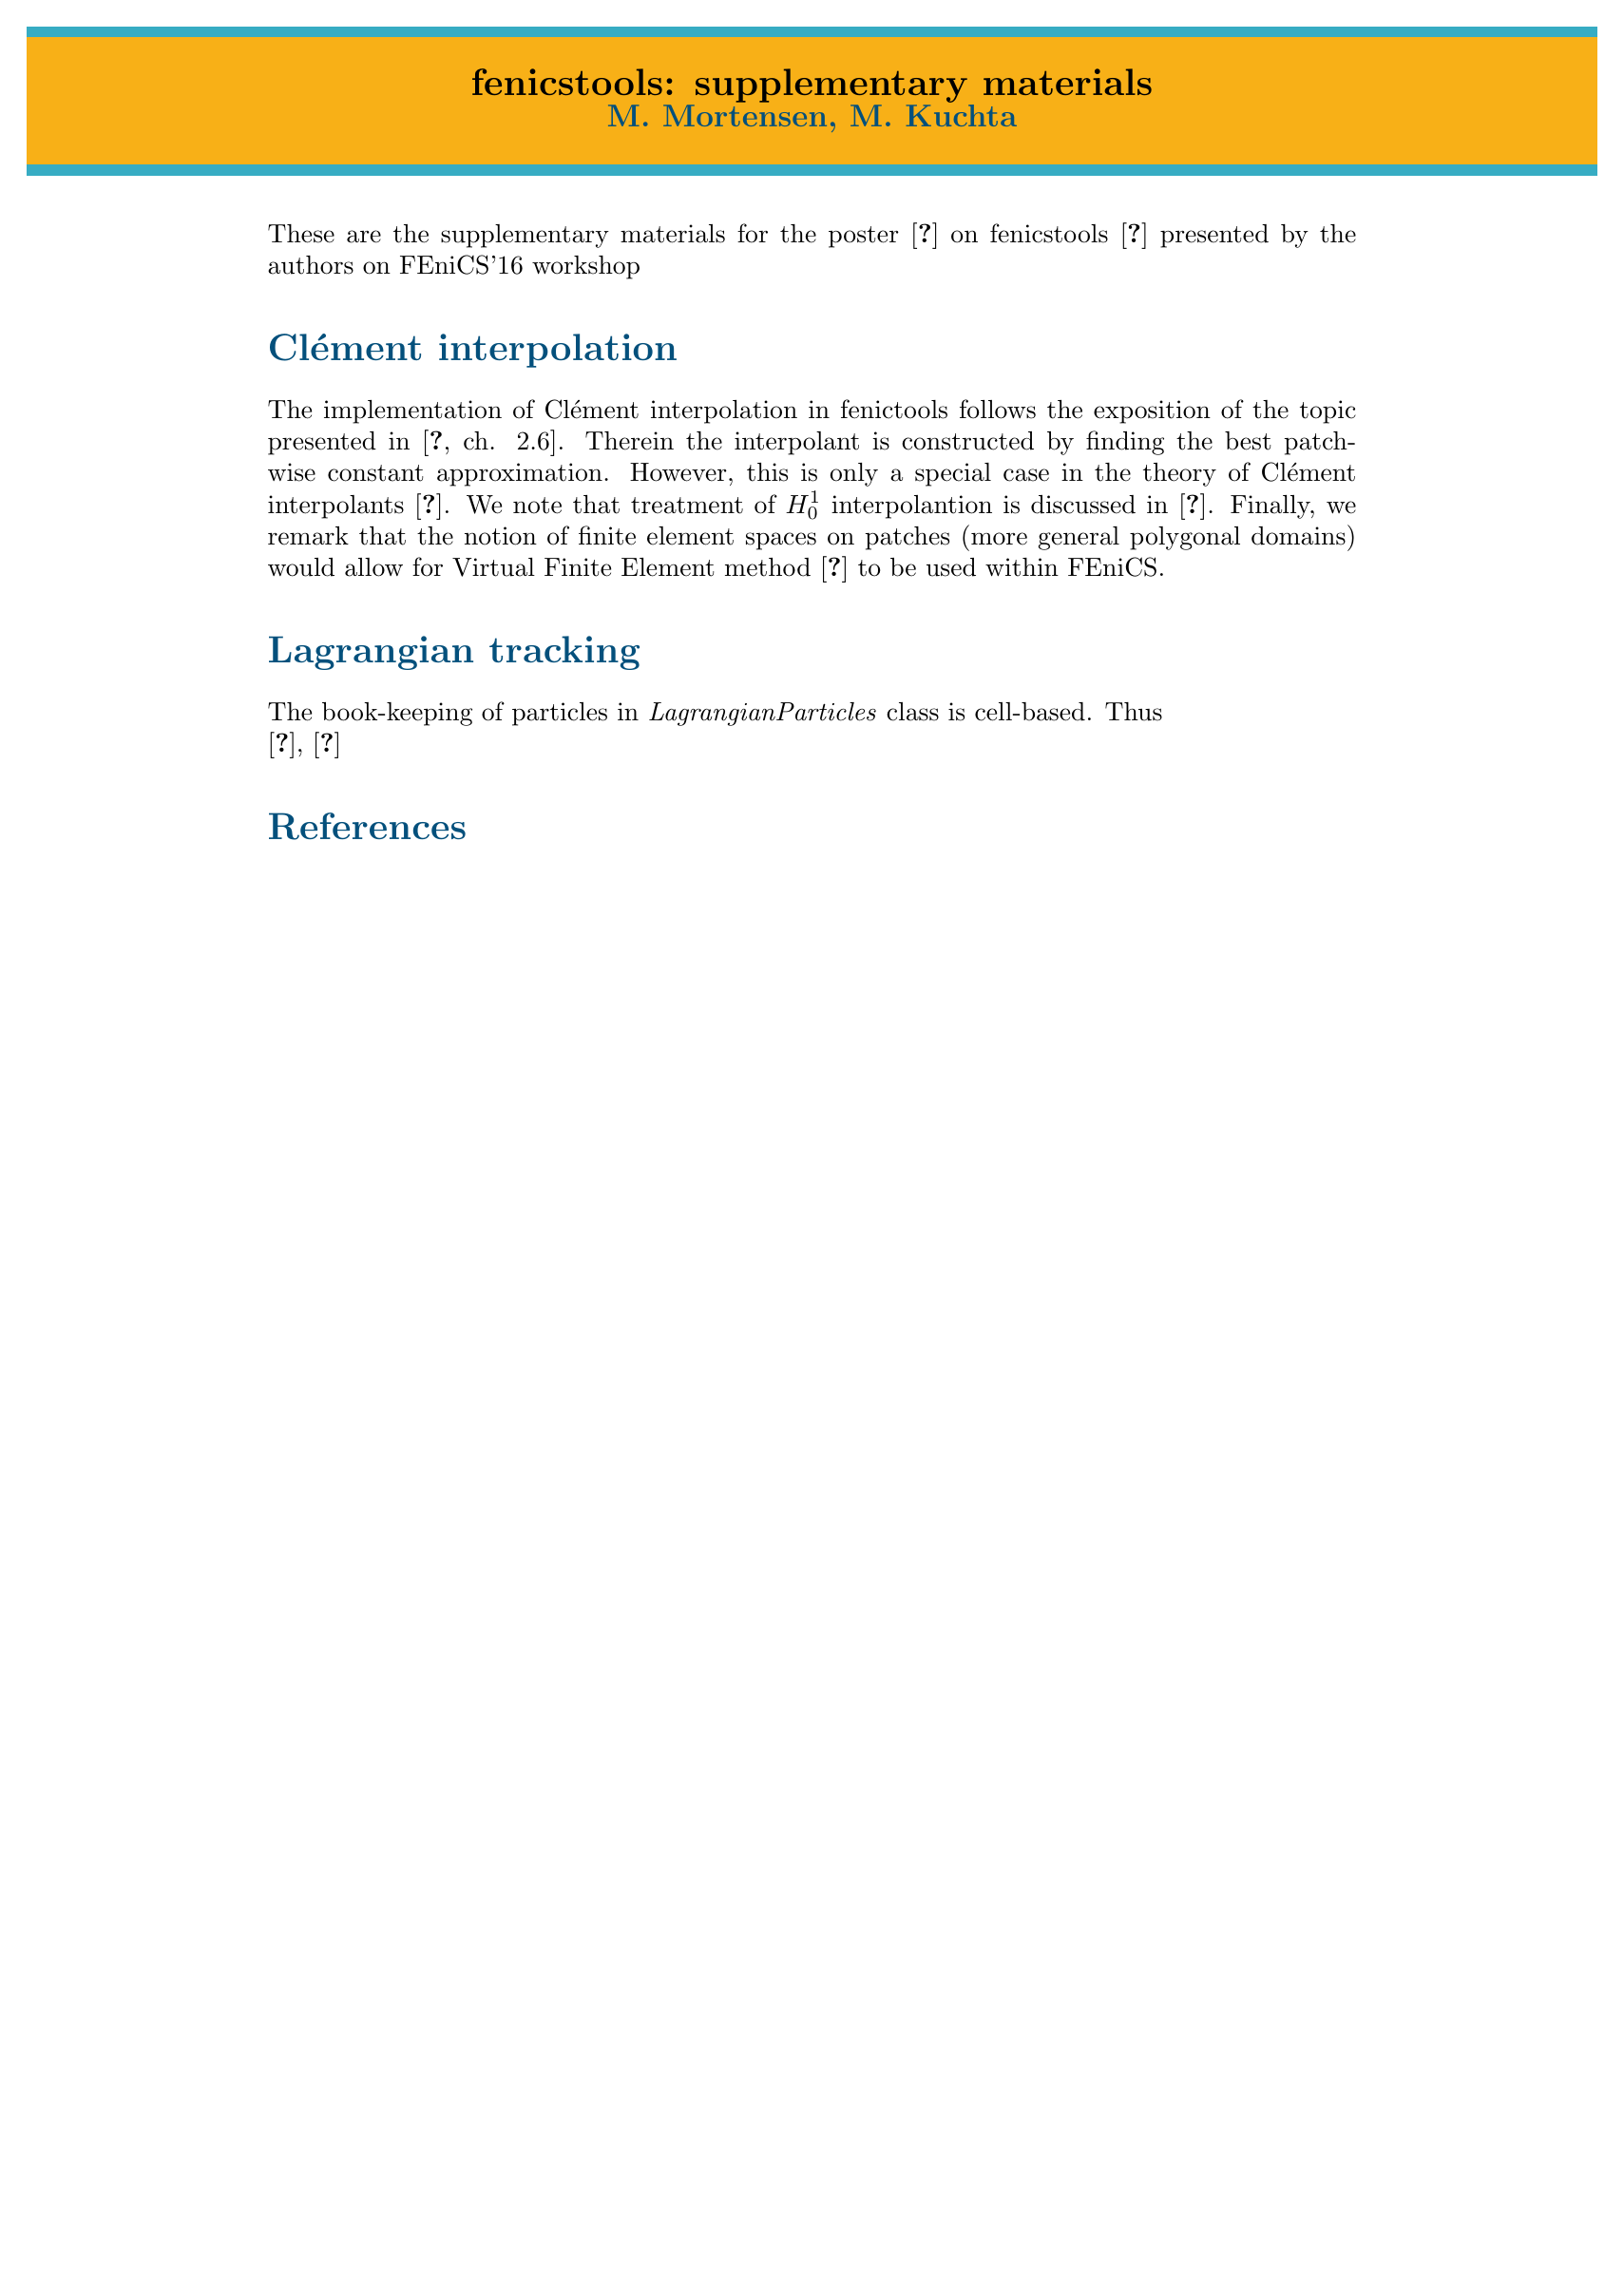
\begin{tikzpicture}[x=21cm, y=29.7cm]
\fill[white, use as bounding box] (0, 0) rectangle (1, 1);

%%%%%%%%%%%%%%%%%%%%%%%%%%
% Title
%%%%%%%%%%%%%%%%%%%%%%%%%%
\begingroup
\draw[fill=eyellow, draw=none] { 
  ($(current bounding box.north west)+(0cm, -20.0mm)$) --
  ($(current bounding box.north east)+(0cm, -20.0mm)$) -- 
  (current bounding box.north east) --
  (current bounding box.north west) -- 
  cycle
};
   %
\draw[elblue, line width=1.5mm]{
  ($(current bounding box.north east)-(0cm, 0.75mm)$) --
  ($(current bounding box.north west)-(0cm, 0.75mm)$)
};
  %
\draw[elblue, line width=1.5mm]{
  ($(current bounding box.north east)+(0cm, -19.25mm)$) --
  ($(current bounding box.north west)+(0cm, -19.25mm)$)
};
\node[anchor=center]
      (title)
      at ($(current bounding box.north)+(0cm, -1.0cm)$)
  {\begin{minipage}{\textwidth}
   \begin{center}
     {\ffmfamily\Large\bfseries\color{black}{fenicstools: supplementary materials}}\\
     {\ffmfamily\large\color{edblue}\textbf{M.~Mortensen, M.~Kuchta}}
   \end{center}
  \end{minipage}};
\endgroup


\node[anchor=north] at ($(current bounding box.north)+(0cm, -2.5cm)$)
{
  \begin{minipage}{1.2\textwidth}
    These are the supplementary materials for the poster \cite{poster} on 
    fenicstools \cite{fenicstools} presented by the authors on FEniCS'16 workshop
  
    \section*{\ffmfamily\color{edblue}{\clm interpolation}}
    The implementation of \clm interpolation in fenictools follows the
    exposition of the topic presented in \cite[ch. 2.6]{braess}. Therein the
    interpolant is constructed by finding the best patch-wise constant
    approximation. However, this is only a special case in the theory of 
    \clm interpolants \cite{clement}. We note that treatment of $H^1_0$
    interpolantion is discussed in \cite{scott}. Finally, we remark that the notion
    of finite element spaces on patches (more general polygonal domains) would allow 
    for Virtual Finite Element method \cite{vfem} to be used within FEniCS.

    % FunctionAssigner

    \section*{\ffmfamily\color{edblue}{Lagrangian tracking}}
    The book-keeping of particles in \emph{LagrangianParticles} class is
    cell-based. Thus

    % Per thomas
    \cite{ptthesis}, \cite{ptpaper}

    \section*{\ffmfamily\color{edblue}{References}}
    \bibliographystyle{plain}
    \bibliography{extras}

  \end{minipage}
};
\end{tikzpicture}
\end{document}
